\begin{problem}[12]{Utilities}

Pacman is buying a raffle ticket from the ghost raffle ticket vendor.
There are two ticket types: $A$ and $B$, but there are multiple specific tickets of each type.  Pacman picks a ticket type, but the ghost will then choose which specific ticket Pacman will receive.  Pacman's utility for a given raffle ticket is equal to the utility of the lottery of outcomes for that raffle ticket. For example, ticket $R_{A,2}$ corresponds to a lottery with equal chances of yielding 10 and 0, and so $U(R_{A,2}) = U([\frac{1}{2}, 10; \frac{1}{2}, 0])$. Pacman, being a rational agent, wants to maximize his expected utility, but the ghost may have other goals! The outcomes are illustrated below.
\begin{figure}[h]
\centering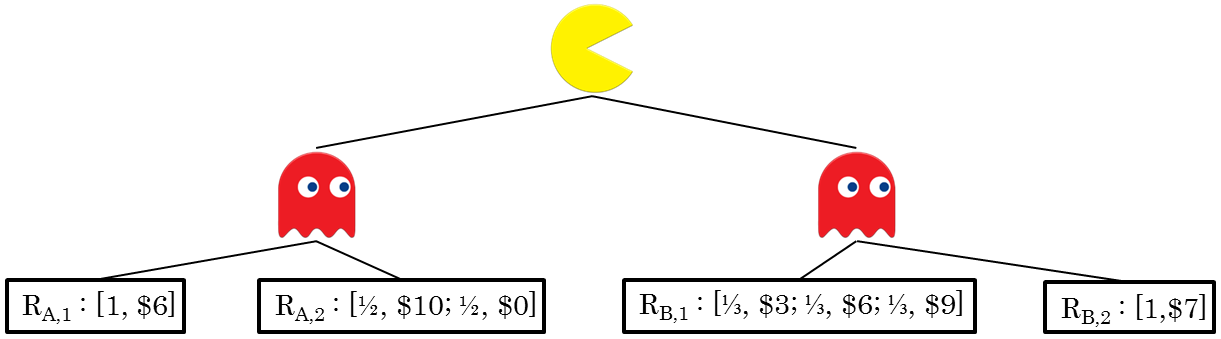
\includegraphics[scale=.5]{figures/utilities.png}
\end{figure}
\vspace{-0.4cm}

\begin{question}[5]{}
Imagine that Pacman's utility for money is $U(m) = m$.
\begin{subquestion}[2]
What are the utilities to Pacman of each raffle ticket?\\
\vspace{.2cm}
{\centering $U(R_{A, 1}) =$ \solution{}{\TwoAiUAOne} \hspace{6cm} $U(R_{A, 2}) =$ \solution{}{\TwoAiUATwo}}\\
\vspace{.2cm}
{\centering $U(R_{B, 1}) =$ \solution{}{\TwoAiUBOne} \hspace{6cm} $U(R_{B, 2}) =$ \solution{}{\TwoAiUBTwo}}\\

\end{subquestion}
\vspace{-0.5cm}
\begin{subquestion}[1]
Which raffle ticket will Pacman receive under optimal play if the ghost is trying to minimize Pacman's utility (and Pacman knows the ghost is doing so)? (circle one)\\
\TwoAii
\end{subquestion}
\begin{subquestion}[2]
What is the equivalent monetary value of raffle ticket $R_{B,1}$?\\
\solution{\vspace{1cm}}{
   \fbox{\begin{minipage}[t][0.6cm][t]{16cm} 2a(iii) answer: \TwoAiii \end{minipage}}\\
}
\end{subquestion}
\end{question}

\begin{question}[5]{}
Now imagine that Pacman's utility for money is given by $U(m) = m^2$. 
\begin{subquestion}[2]
What are the utilities to Pacman of each raffle ticket?\\
\vspace{.2cm}
{\centering $U(R_{A, 1}) =$ \solution{}{\TwoBiUAOne} \hspace{6cm} $U(R_{A, 2}) =$ \solution{}{\TwoBiUATwo}}\\
\vspace{.2cm}
{\centering $U(R_{B, 1}) =$ \solution{}{\TwoBiUBOne} \hspace{6cm} $U(R_{B, 2}) =$ \solution{}{\TwoBiUBTwo}}\\
\end{subquestion}
\vspace{-0.5cm}
\begin{subquestion}[1]
The ghost is still trying to minimize Pacman's utility, but the ghost mistakenly thinks that Pacman's utility is given my $U(m) = m$, and Pacman is aware of this flaw in the ghost's model.  Which raffle ticket will Pacman receive? (circle one)\\
\TwoBii
\end{subquestion}
\begin{subquestion}[2]
What is the equivalent monetary value of raffle ticket $R_{B,1}$?\\
\solution{\vspace{1cm}}{
   \fbox{\begin{minipage}[t][0.6cm][t]{16cm} 2b(iii) answer: \TwoBiii \end{minipage}}\
}
\end{subquestion}
\end{question}

\begin{question}[2]{}
Pacman has the raffle with distribution [0.5, \$100; 0.5, \$0]. A ghost insurance dealer offers Pacman an insurance policy where Pacman will get \$100 regardless of what the outcome of the ticket is. If Pacman's utility for money is $U(m) = \sqrt{m}$, what is the maximum amount of money Pacman would pay for this insurance? \\
\solution{\vspace{3cm}}{
   \fbox{\begin{minipage}[t][2.6cm][t]{17cm} 2c answer: \TwoC \end{minipage}}\
}
\end{question}
\end{problem}
